

\section{Introduction}
% The very first letter is a 2 line initial drop letter followed
% by the rest of the first word in caps.
% 
% form to use if the first word consists of a single letter:
% \IEEEPARstart{A}{demo} file is ....
% 
% form to use if you need the single drop letter followed by
% normal text (unknown if ever used by IEEE):
% \IEEEPARstart{A}{}demo file is ....
% 
% Some journals put the first two words in caps:
% \IEEEPARstart{T}{his demo} file is ....
% 
% Here we have the typical use of a "T" for an initial drop letter
% and "HIS" in caps to complete the first word.
\IEEEPARstart{A}{ well-designed} graph is a powerful tool 
that transends barriers of language to
communicate complex concepts from author to audience. It becomes a 
problem if readers are unable to easily extract the main message, especially
when distortion is encoded. The source of a distortion may be due to 
intrinsic deformities in the graph or simply the perceptual limitations of
the audience. Examples include Tufte's \emph{Lie-Factor} \cite[p. 57--69]{tufte} in which the proportion of the physical space occupied by the graphic is 
inconsistent with underlying data; calculated ratio (of proportions) less than one indicate 
underrepresentation. Another example is the M\"{u}ller-Lyer family of illusions such as the sine wave, where viewers perceive extents at the curves to be of different height than in the straight regions even though all regions were of the same height \cite{day:1991}.

Regardless of the cause of distortion, the graph author has a duty to create visualizations that
 allows readers to extract an accurate interpretation of the underlying data. The \emph{Lie-Factor}
provides a quantitative method to evaluate distortion due to graph deformities. In order to ascertain the
impact of distortion due to perceptual limits, usability studies provide empirical evidence supporting 
underlying metaphorical models both known and unpredicted.  This paper presents a method for developing new statistical visualization which incoporates usablity testing, a technique borrowed from 
the field of user centered design. It is our belief that the results of such testing allows a graph author
to make design choices to reduce distortion due to perceptual limits. We describe how a routine user study 
during development of parallel coordinates for categorical data led to the unexpected and unpredicted discovery of the \emph{line-width} illusion. We introduce the {\it common-angle plot} as an alternative  method for displaying categorical data in a manner that minimizes the effect from perceptual illusions.
The display preserves properties of parallel coordinates, such as the potential to visualize a large number of dimensions simultaneously, but also presents frequency information. 
Finally, we present results from user studies as evidence that common angle plots resolve the problem of the line width illusion. 
% You must have at least 2 lines in the paragraph with the drop letter
% (should never be an issue)

\section{Related Work}
This section describes a selection of related work as context for the contributions 
presented here.

\subsection{Line width illusion}




\begin{figure}
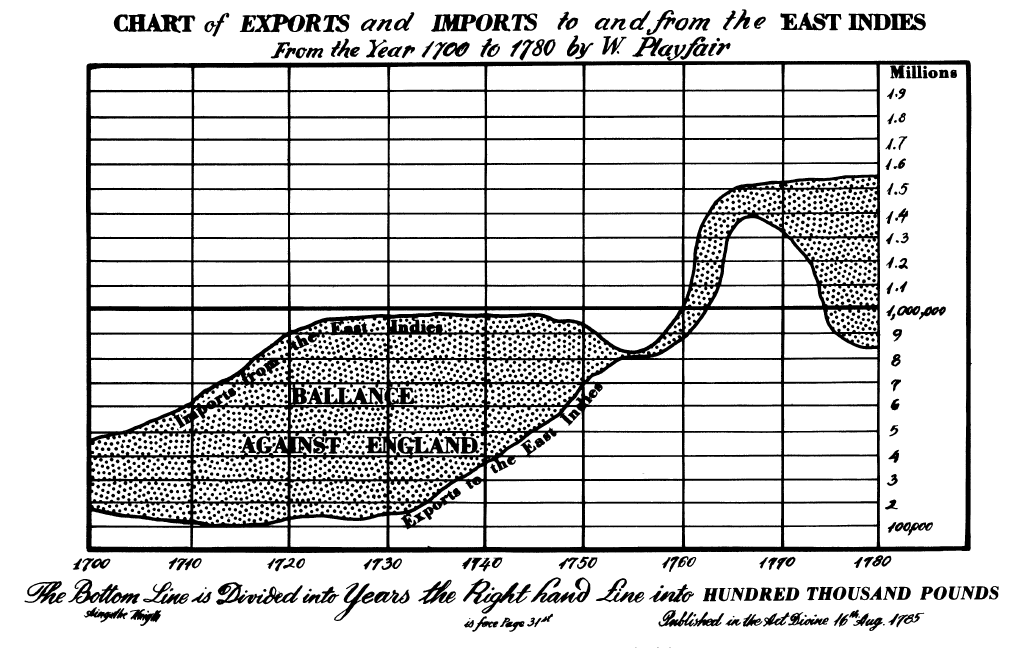
\includegraphics[width=.9\linewidth]{images/playfair_east_indies_gross}
\caption{\label{playfair}
Playfair's chart from the Commercial and Political Atlas (1786) showing the balance of trade between England and the East Indies.  In which years was the difference between imports and exports the highest? }
\end{figure}
An example of the  {\it line width illusion} is displayed in  figure  \ref{playfair}. This chart displays the balance of trade between England and the East Indies as shown by William Playfair in his Commercial and Political Atlas, 1786 \cite{playfair, playfair2}.  One purpose of this chart is to demonstrate the difference between imports and exports in a particular year and its pattern over that time frame. The difference in exports and imports is encoded as the vertical difference between the lines. When observers are asked to sketch out the difference between exports and imports  \cite{cleveland:1984}, they very often  miss the steep rise in the difference between the lines in the years between about 1755 and 1765. Figure \ref{playfair2} shows the  actual difference between imports and exports. 



\begin{figure}
\centering
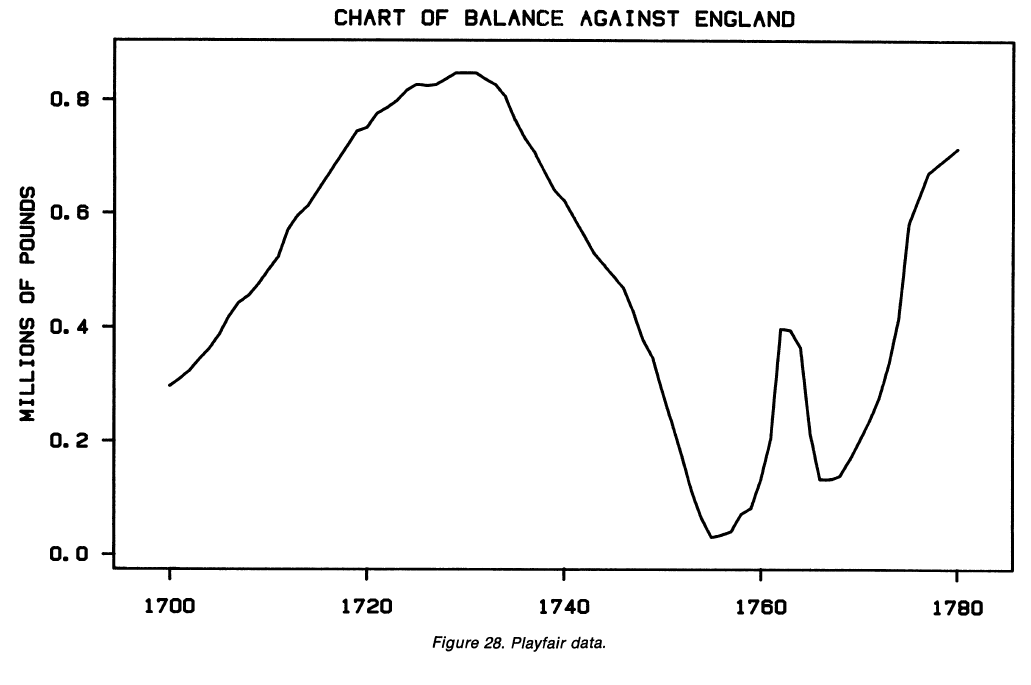
\includegraphics[width=.8\linewidth, height=.4\linewidth]{images/playfair_differenz_cleveland}
\caption{\label{playfair2}
Difference between exports and imports from England to and from the East Indies in the 18th century -- the steep rise in the difference around 1760  comes as a surprise to many viewers of the raw data in figure \ref{playfair}.  }
\end{figure}


This phenomenon  is known and widely discussed in statistical graphics literature \cite{cleveland:1984, tufte, wainer:2000, robbins:2005}. It  is due to our  tendency to assess distance between curves as the minimal (orthogonal) distance rather than the  vertical distance -- see sketch \ref{fig:linewidth} for a visual representation of both.


In the perception literature, this phenomenon is known as part of a group of geometrical optical misperceptions of a context-sensitive nature classified as M\"uller-Lyer illusions \cite{day:1991}. Interestingly, there seems to be a general agreement that this illusion exists, but a quantification of it is curiously absent from literature. 

The type of chart as shown in figure~\ref{playfair} proposed by Playfair is shown quite commonly, particular in election years -- where these kind of charts are used to enable comparisons of support for several candidates, the recommendation from literature is to avoid charts in which the audience is asked to do visual subtractions, and show these differences directly.

\subsection{Parallel sets}

Parallel sets (parsets) have been introduced by R Kosara \cite{kosara:2006} as one way to visualize multivariate categorical data. Since their initial publication, they have spread to mass media outlets: see e.g. 
``How to understand risk in 13 clicks," BBC \cite{bbc:2009}.

  While retaining the %independent 
ability to visualize a large number of dimensions simultaneously that is the parallel coordinates' hallmark trade, parallel sets introduce the frequency scale that is a well-known feature of other categorical displays such as barcharts or mosaic plots \cite{hartigan:1981, friendly:1992, hofmann:2000, theus:1997}.
 Initially, frequencies of categories  were displayed as stacked boxes; in  later versions of parallel sets the boxes are reduced to simple lines \cite{parsetredesign}. Various implementations of parallel sets exist besides the original Java version of Eagereyes \cite{eagereyes}, e.g.  J Davies introduced a d3 \cite{d3} version in  \cite{davies}.  


\begin{figure}[hbtp]
\centering
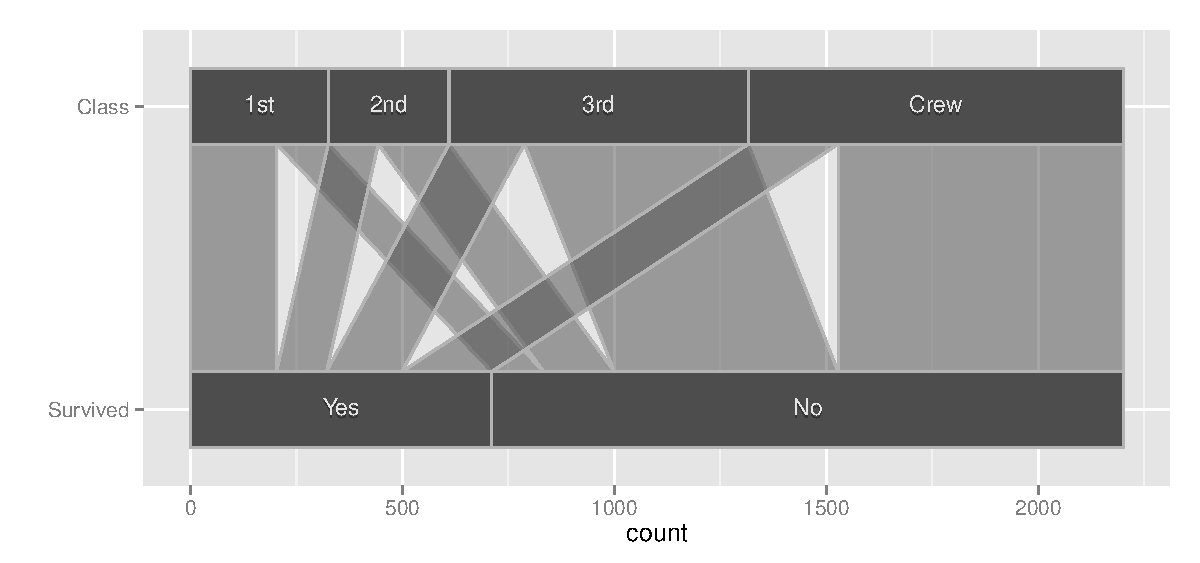
\includegraphics[width=.9\linewidth]{images/parset-titanic}
\caption{\label{question1a} Parallel sets plot showing the relationship between survival of the sinking of the HMS Titanic and class membership. }
\end{figure}
%XXX Description of parallel sets - and example


%%XXX PS and line-width illusion
Figure \ref{question1a} gives an example for a two dimensional parallel sets plot investigating the relationship between class status and survival on board the HMS Titanic  \cite{dawson:1995}. Class status is recorded as either crew member or passengers in  first, second, or third class. 

 The top bar in figure \ref{question1a} shows the  variable Class. The bottom bar shows survival  as yes and no. Between the bars lines are drawn to visualize the relationship between class membership and  survival. 
  Based on the number of survivor and non survivors
  these bands are drawn from each class, and their (horizontal) width is proportional to the number of people they represent. 
%XXX PS and line-width illusion


%
\subsection{Strength of  line width illusion}\label{distortion}

%The difference between perceived and actual line width 
When visually evaluating lines of thickness greater than one, the line width illusion applies, only now the {\it edges} of a single line  take on the role of the separate curves. %in the parallel sets 
As above, there is a strong preference of evaluating the width of lines orthogonal to their slopes as opposed to horizontally (see figure \ref{fig:linewidth})  needed for a correct  evaluation of parsets-style displays.

Orthogonal $w_o$ and horizontal $w_h$ line widths are related -- the orthogonal line width depends on the angle (or, equivalently, the slope) of the line:
\begin{equation}\label{adjust}
w_o = w_h \sin \theta,
\end{equation}
where $\theta$ is the angle of the line with respect to the horizontal line.

\begin{figure}[htbp]
\begin{center}
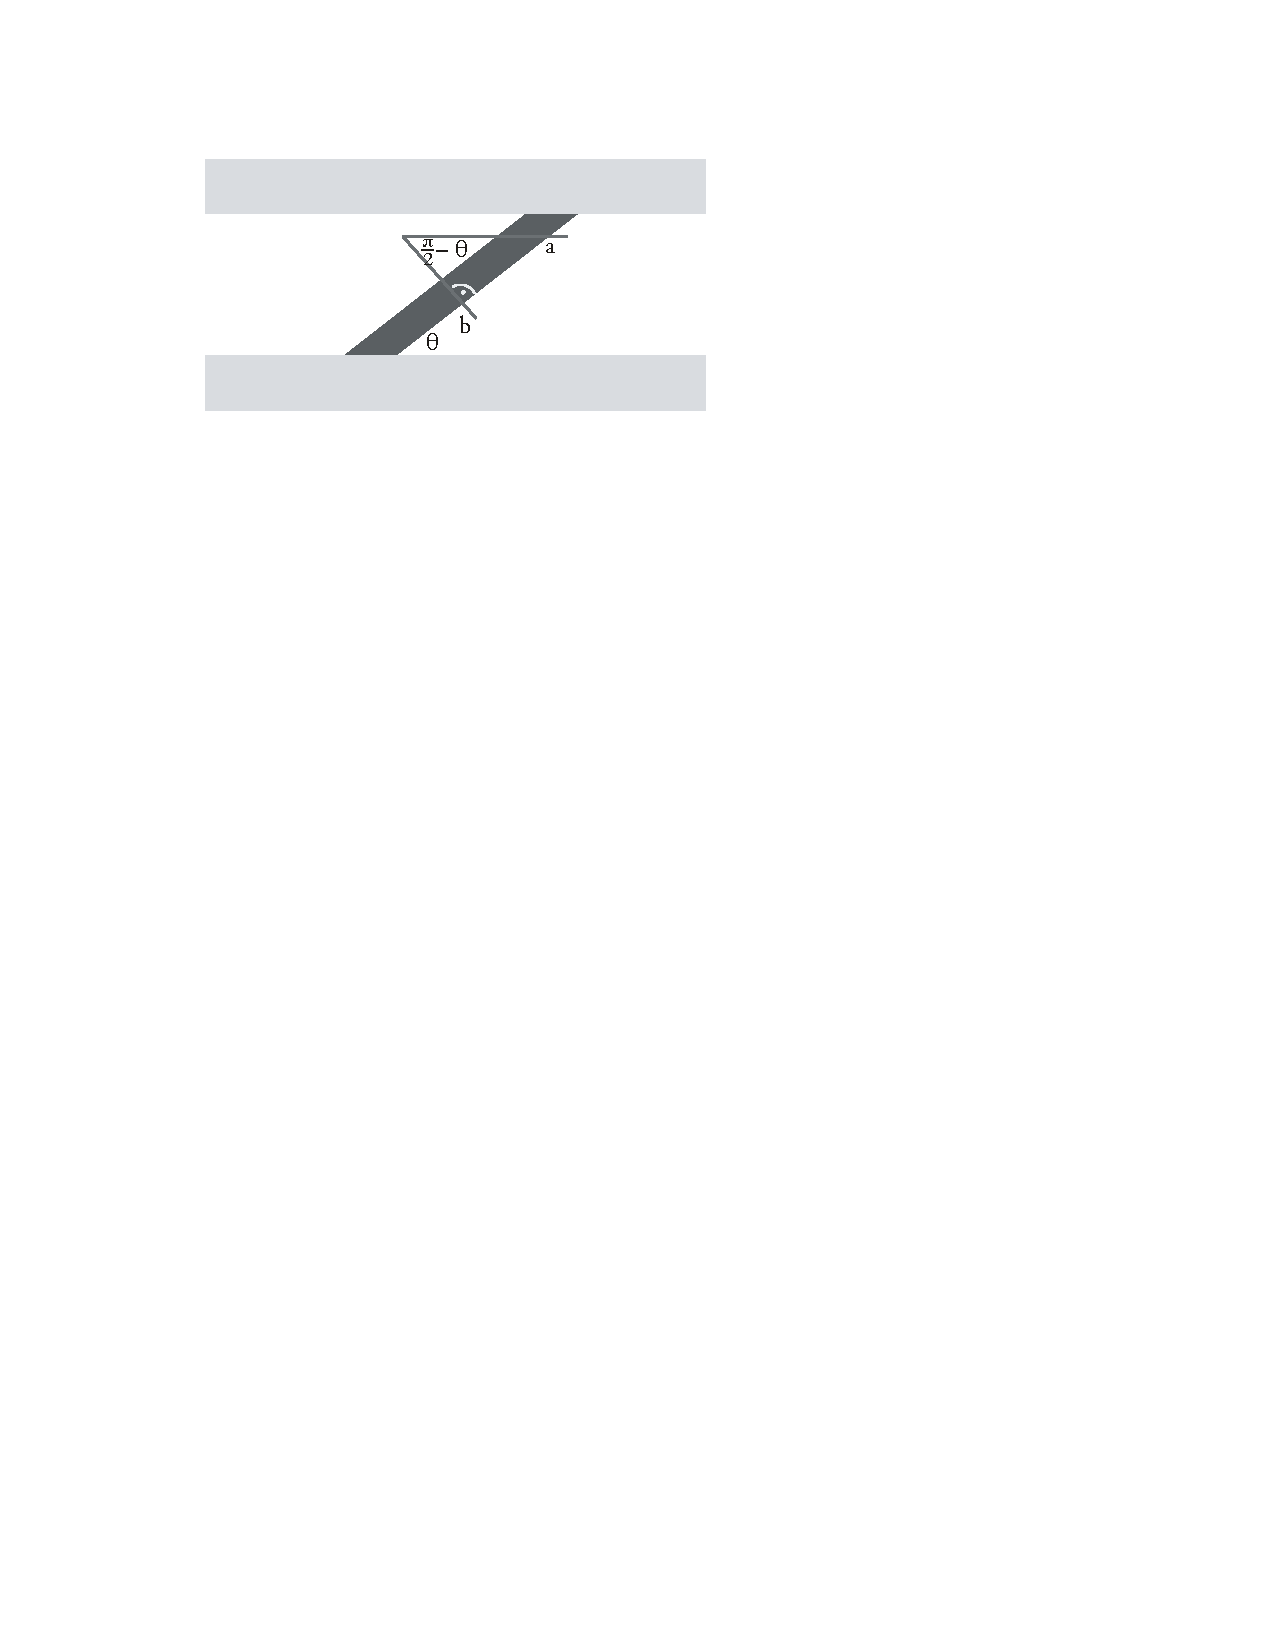
\includegraphics[width=0.6\linewidth]{images/linewidth}
\end{center}
\caption{\label{fig:linewidth}Sketch of line width assessments: (a) is showing  horizontal width, (b) shows  width orthogonal to the slope. Survey results in section \ref{results}  indicate that observers associate line width more with  orthogonal width (b) than horizontal width (a).}
\end{figure}



%XXX aspect ratio


\begin{figure*}[htbp]
\begin{center}
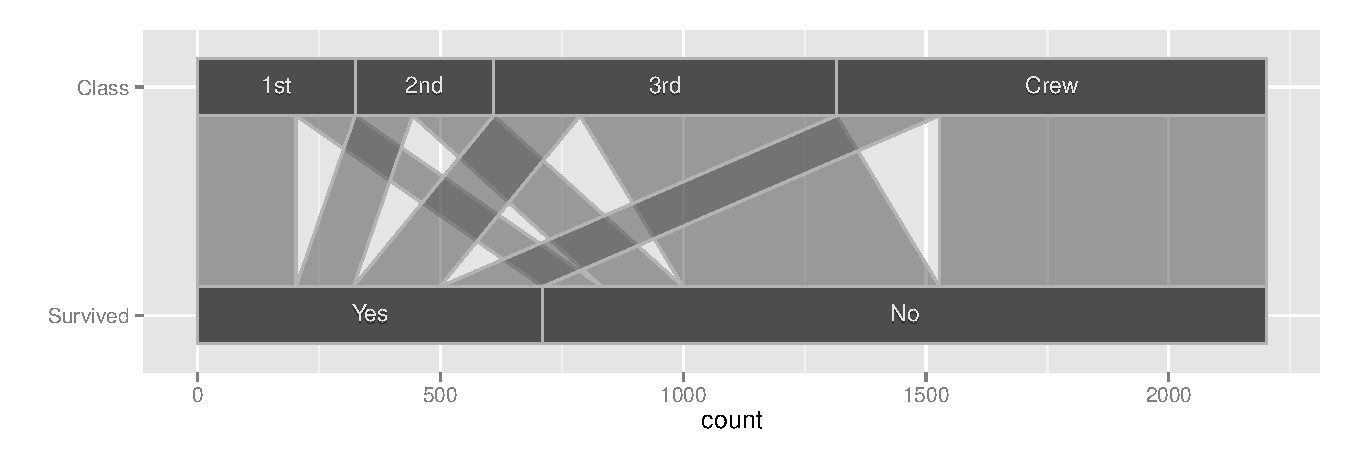
\includegraphics[height=1.5in]{images/aspect31-titanic.pdf}
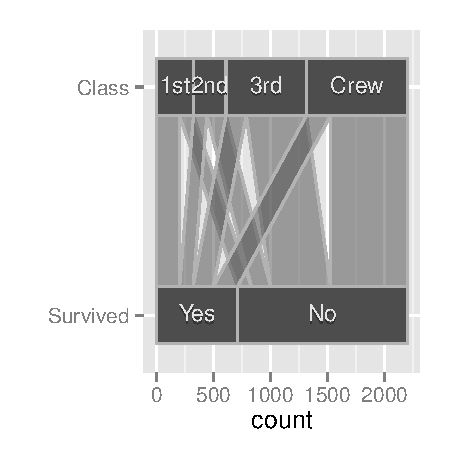
\includegraphics[height=1.5in]{images/aspect33-titanic.pdf}
\end{center}
\caption{\label{fig:aspect}Parallel sets plots of survival on the Titanic by class. Different aspect ratios  seemingly change the thickness of line segments, compare e.g. number of survivors in 3rd class and in the crew. }
\end{figure*}



The perceived slope of a line very much depends on the aspect ratio of the corresponding plot -- changing the height to width ratio of a display  will change our perception of the corresponding line widths, if they are not adjusted for the slope \cite{cleveland:1984}. This finding is not new, but its strength on our perception is surprising, as can be seen in the example of  figure \ref{fig:aspect}.  Again, survival and class membership on the Titanic is shown; the same parallel sets plot is shown twice in this figure, but with very different aspect ratios: in the  plot on the left the number of surviving 3rd class passengers seems to be about twice as big as the number of survivors among crew members, whereas in the plot on the right the lines have about equal (orthogonal) width. Obviously, this is not due to a change in numbers.

For parsets-style displays, the audience has {\it area of the line segment} an alternate visual cue when evaluating frequencies. Because height (or width for a rotated display) of  line segments is constant across the display, the width of a particular  segment is proportional to its area. We can therefore employ area comparisons as a proxy or to augment line width evaluations. 
However, existing literature suggests that this method of comparison is particularly  prone to errors in two scenarios commonly seen in parallel sets: (1) extreme aspect ratios of the rectangular shape \cite{heer:2010} %occupied by thick line segments 
and (2) when comparing rectangles rotated relative to each other \cite{kong:2010}. 
This incorrect perception and comparison of areas distorts the message readers discern from the graph. %additional contextual evidence that reinforce and strengthen distortion introduced by the line width illusion.


% needed in second column of first page if using \IEEEpubid
%\IEEEpubidadjcol
\subsection{Hammock plots}
%XXX Description of hammock plots and example

Hammock plots, introduced by M Schonlau in \cite{schonlau:2003}, provide an alternative to parallel sets that is adjusted for the line width illusion. This is done by  adjusting the --horizontal-- line width by  a factor of $\sin \theta$, as discussed in equation (\ref{adjust}). This adjustment makes the perceived --orthogonal-- line width to be proportional to the number of observations it represents. 
 Figure \ref{hammock} shows an example of a four dimensional hammock plot of the Titanic data. From top to bottom Class, Gender, Survival, and again Class are shown. 
\begin{figure}
%cols <- c(brewer.pal(name="Blues", 6)[-c(1,2)], rev(brewer.pal(name="Oranges", 3)[-1]), rev(brewer.pal(name="Greens",3)[-1]))
%ggparallel(names(titanic)[c(1,4,2,1)], order=c(0,1,1,0), method="hammock", ratio=.25, text.angle=0, titanic, weight="Freq") +
%  scale_fill_manual(values=cols, guide="none") +
%  scale_colour_manual(values=cols, guide="none") + coord_flip() 
%ggsave("hammock-titanic.pdf", width=6, height=8)
\centering
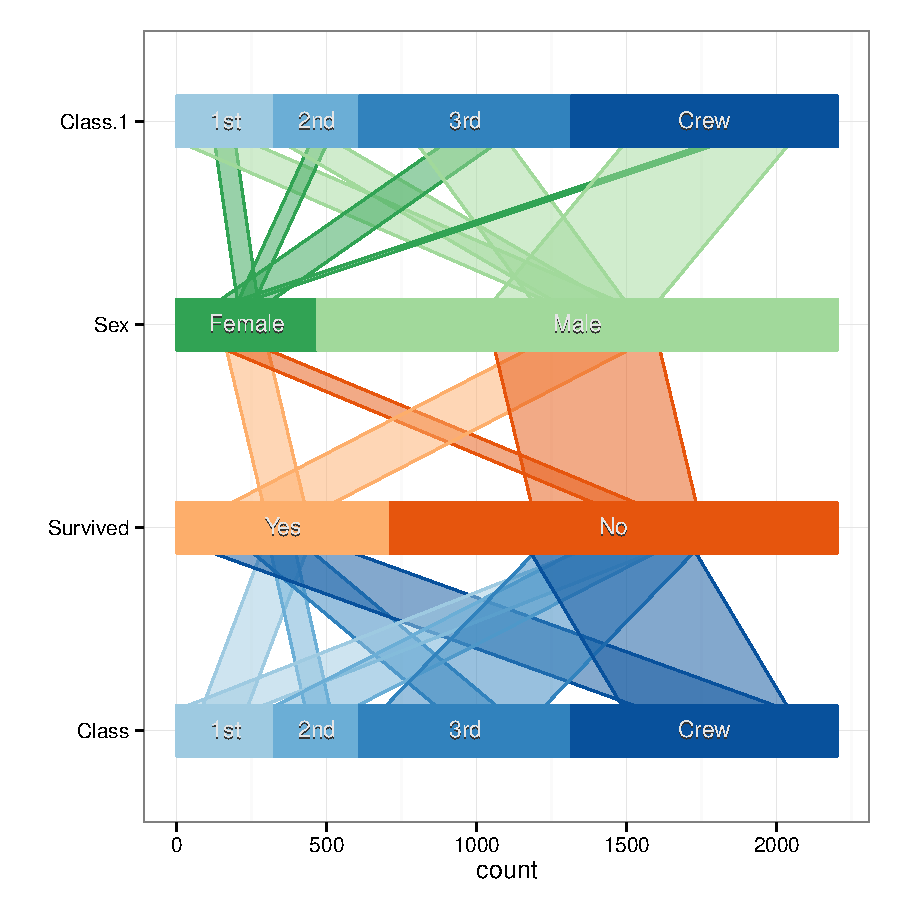
\includegraphics[width=\linewidth]{images/hammock-titanic}
\caption{\label{hammock} Hammock plot of the relationship between Class and Survival on the Titanic. }
\end{figure}

Similarly to the parallel sets plot, the bars are divided according to class membership numbers.  Lines connect categories between neighboring variables, orthogonal line widths are representing the number of individuals in each combination. Unlike the parallel sets, the lines start from the middle of the bin and connect to the middle of the other variable's bins. 

The graph shows that barely any women were in the crew, while male crew members make up the second largest contingent overall. Overall a few more men survived than women. Proportionally the situation is much different -- a much higher percentage of women survived than men. While more first class passengers survived than not, the  survival chances of second class passengers were about fifty-fifty. For third class passengers and crew members fewer members did  survive than not. 

As the adjustment of line widths is made with respect to the angle $\theta$, which itself depends on the aspect ratio of a plot, we need complete control over these properties of the plotting device when constructing hammock plots  -- in our implementation (see below for details) we have dealt with this issue by fixing the aspect ratio. This is problematic in some situations, where the rendering has to be done without knowledge of the plotting device. 

Another problem that arises in evaluating hammock plots is that if an observer focuses on horizontal line width  the plots suffer from a {\it reverse line width illusion}:  judging the number of survivors by class in figure \ref{hammock} based on horizontal line width  results in an ordering of (largest to smallest) Crew, 3rd, 1st, and 2nd -- which is not correct either. Using horizontal width is inviting, since the lines are centered around the middle of a level, facilitating this  comparison. 

\section{Overview}
From previous work \cite{cleveland:1984, tufte, wainer:2000, robbins:2005, heer:2010, kong:2010}, we may conclude that numerically accurate representations of data
are subject to distortion due to perceptual limitations. In particular,
the width of a single line of some thickness or the distance between two lines of minimal thickness is 
subject to the \emph{line width illusion} even though the depiction is numerically sound.
 Furthermore, design choices during implementation \cite{schonlau:2003} may
reduce the impact of such limitations.

Before describing our method for identifying and resolving perceptual limitations during the 
design phase of creating a new data chart, we review the design goal: extending parallel coordinates 
for application to categorical data. Parallel coordinates were introduced to visualize large numbers of numeric variables. 
Recent adaptations of parallel coordinates  \cite{ kosara:2006, bendix:2005, leblanc:1990, 
spenke:2003, schonlau:2003} and other, frequency-based, methods to display categorical data, such as mosaic plots  \cite{hartigan:1981, friendly:1992, hofmann:2000, theus:1997},  have addressed perceptual constraints \cite{cleveland:1984} at a theoretical level, but lack reporting of human subjects testing as validation. 

\section{Common angles}
\section{Usability Testing}
\subsection{Test}
\subsection{Results}

% An example of a floating figure using the graphicx package.
% Note that \label must occur AFTER (or within) \caption.
% For figures, \caption should occur after the \includegraphics.
% Note that IEEEtran v1.7 and later has special internal code that
% is designed to preserve the operation of \label within \caption
% even when the captionsoff option is in effect. However, because
% of issues like this, it may be the safest practice to put all your
% \label just after \caption rather than within \caption{}.
%
% Reminder: the "draftcls" or "draftclsnofoot", not "draft", class
% option should be used if it is desired that the figures are to be
% displayed while in draft mode.
%
%\begin{figure}[!t]
%\centering
%\includegraphics[width=2.5in]{myfigure}
% where an .eps filename suffix will be assumed under latex, 
% and a .pdf suffix will be assumed for pdflatex; or what has been declared
% via \DeclareGraphicsExtensions.
%\caption{Simulation Results.}
%\label{fig_sim}
%\end{figure}

% Note that IEEE typically puts floats only at the top, even when this
% results in a large percentage of a column being occupied by floats.


% An example of a double column floating figure using two subfigures.
% (The subfig.sty package must be loaded for this to work.)
% The subfigure \label commands are set within each subfloat command,
% and the \label for the overall figure must come after \caption.
% \hfil is used as a separator to get equal spacing.
% Watch out that the combined width of all the subfigures on a 
% line do not exceed the text width or a line break will occur.
%
%\begin{figure*}[!t]
%\centering
%\subfloat[Case I]{\includegraphics[width=2.5in]{box}%
%\label{fig_first_case}}
%\hfil
%\subfloat[Case II]{\includegraphics[width=2.5in]{box}%
%\label{fig_second_case}}
%\caption{Simulation results.}
%\label{fig_sim}
%\end{figure*}
%
% Note that often IEEE papers with subfigures do not employ subfigure
% captions (using the optional argument to \subfloat[]), but instead will
% reference/describe all of them (a), (b), etc., within the main caption.


% An example of a floating table. Note that, for IEEE style tables, the 
% \caption command should come BEFORE the table. Table text will default to
% \footnotesize as IEEE normally uses this smaller font for tables.
% The \label must come after \caption as always.
%
%\begin{table}[!t]
%% increase table row spacing, adjust to taste
%\renewcommand{\arraystretch}{1.3}
% if using array.sty, it might be a good idea to tweak the value of
% \extrarowheight as needed to properly center the text within the cells
%\caption{An Example of a Table}
%\label{table_example}
%\centering
%% Some packages, such as MDW tools, offer better commands for making tables
%% than the plain LaTeX2e tabular which is used here.
%\begin{tabular}{|c||c|}
%\hline
%One & Two\\
%\hline
%Three & Four\\
%\hline
%\end{tabular}
%\end{table}


% Note that IEEE does not put floats in the very first column - or typically
% anywhere on the first page for that matter. Also, in-text middle ("here")
% positioning is not used. Most IEEE journals use top floats exclusively.
% Note that, LaTeX2e, unlike IEEE journals, places footnotes above bottom
% floats. This can be corrected via the \fnbelowfloat command of the
% stfloats package.



\section{Conclusion}
The conclusion goes here.





% if have a single appendix:
%\appendix[Proof of the Zonklar Equations]
% or
%\appendix  % for no appendix heading
% do not use \section anymore after \appendix, only \section*
% is possibly needed

% use appendices with more than one appendix
% then use \section to start each appendix
% you must declare a \section before using any
% \subsection or using \label (\appendices by itself
% starts a section numbered zero.)
%


\appendices
%\section{Proof of the First Zonklar Equation}
%Appendix one text goes here.
%
%% you can choose not to have a title for an appendix
%% if you want by leaving the argument blank
%\section{}
%Appendix two text goes here.


% use section* for acknowledgement
\section*{Acknowledgment}


The survey for this study was carried out with approval from  IRB-ID 12-204.


% Can use something like this to put references on a page
% by themselves when using endfloat and the captionsoff option.
\ifCLASSOPTIONcaptionsoff
  \newpage
\fi



% trigger a \newpage just before the given reference
% number - used to balance the columns on the last page
% adjust value as needed - may need to be readjusted if
% the document is modified later
%\IEEEtriggeratref{8}
% The "triggered" command can be changed if desired:
%\IEEEtriggercmd{\enlargethispage{-5in}}
